\apendice{Especificación de Requisitos}

\section{Introducción}

En este anexo se recogen las especificaciones de requisitos requeridas para este proyecto. Estas definirán el comportamiento esperado del sistema. 

\section{Objetivos generales}

En este proyecto se ha tratado de llevar a cabo los siguientes objetivos de carácter general: 

\begin{itemize}
\item Diseñar un \emph{drone} capaz de recorrer un espacio, en el que existan obstáculos, de forma segura.
\item Diseñar un sistema de acceso al \emph{drone} de forma segura. Tanto para controlarlo de forma remota, como para activar los mecanismos de control automatizados.
\item Diseñar una interfaz web que permita la visualización en tiempo real de la cámara del \emph{drone}, así como su control remoto por un operador.
\end{itemize}


\section{Catálogo de requisitos}
Los siguientes requisitos se derivan de los objetivos generales arriba dispuestos: 

\subsubsection{Requisitos Funcionales}
\begin{itemize}
\item[\textbf{RF-1}] Acceso al sistema: El usuario debe poder iniciar sesión en el sistema.

\item[\textbf{RF-2}] Cierre de sesión: El usuario debe poder cerrar sesión en el sistema.

\item[\textbf{RF-3}] Gestión del sistema: El usuario debe ser capaz de gestionar el sistema completo que hay a bordo del \emph{drone}.

	\begin{itemize}

			\item[\textit{RF-3.1}] Gestión del \emph{streaming} de vídeo: El usuario debe poder iniciar/detener el streaming de vídeo.
			\item[\textit{RF-3.2}] Grabaciones de vídeo: El usuario debe poder iniciar/detener y descargar las grabaciones de vídeo.
			\item[\textit{RF-3.3}] Gestión de controles del \emph{drone}: El usuario debe poder activar/desactivar el control manual del dispositivo.
				\begin{itemize}
					\item[RF-3.3.1] Seguridad automatizada: El \emph{drone} debe presentar mecanismos de autopreservación. Debe protegerse frente a obstáculos.
				\end{itemize}
			\item[\textit{RF-3.4}] Gestión de control automático del \emph{drone}: El usuario debe poder activar/desactivar los mecanismos de control automatizado.

		\item[\textit{RF-3.5}] Registro de acciones: Las acciones llevadas a cabo por el usuario deben guardarse en un registro.
		\end{itemize}
		
\item[\textbf{RF-4}] Gestión del \emph{backend}: El usuario debe poder acceder al equipo que controla el \emph{backend}.
			\begin{itemize}
				\item[\textit{RF-4.1}] Gestión del sistema operativo: El usuario debe poder llevar a cabo las tareas de gestión del sistema operativo como crea conveniente.
			\end{itemize}		
	

\item[\textbf{RF-5}] Registro de sucesos: Intentos de intrusión deben ser registrados.

\item[\textbf{RF-6}] Reconocimiento de dispositivos: La aplicación web debe ser capaz de reconocer un dispositivo (\emph{joystick} o emisora) conectado al equipo, para llevar a cabo el control del \emph{drone}.


\end{itemize}


\subsubsection{Requisitos no funcionales}
\begin{itemize}
\item[\textbf{RNF-1}] Usabilidad: El \emph{frontend} ha de ser sencillo de utilizar e intuitivo. En el caso de producirse errores, estos deben ser claramente explicados, o registrados.
\item[\textbf{RNF-2}] Rendimiento: Tanto el \emph{frontend}, como el \emph{backend} deben funcionar de forma eficiente. Retardos elevados podrían dar lugar a problemas muy serios en la ejecución de las ordenes del usuario.
\item[\textbf{RNF-3}] Capacidad y Escalabilidad: Tanto el \emph{frontend} como el \emph{backend} deben ser escalables. El \emph{frontend} debe ser capaz de soportar una asiduidad grande de usuarios, así como permitir añadir múltiples agentes a cada usuario. El \emph{backend}, debe permitir añadir controladores sin que haya que reestructurar todo el sistema.
\item[\textbf{RNF-4}] Disponibilidad: El sistema al completo debe ser robusto. El \emph{frontend} debe estar disponible para su uso el mayor tiempo que sea posible. El \emph{backend} debe ser capaz de recuperarse de errores, y determinar acciones a tomar en el caso de que se produzcan.
\item[\textbf{RNF-5}] Seguridad: Tanto el acceso al \emph{frontend} como al \emph{backend} deben hacerse de forma segura. En ningún momento el \emph{drone} debe guardar imágenes de la zona vigilada. El almacenamiento de contraseñas se hará de forma cifrada, y la comunicación entre el \emph{backend} y el \emph{frontend} deberá ser segura.
\end{itemize}

\section{Especificación de requisitos}

Esta sección detallará el diagrama de casos de uso, y detallará cada uno de ellos. 



\afterpage{
\clearpage
\begin{landscape}
\begin{figure}
	\centering
	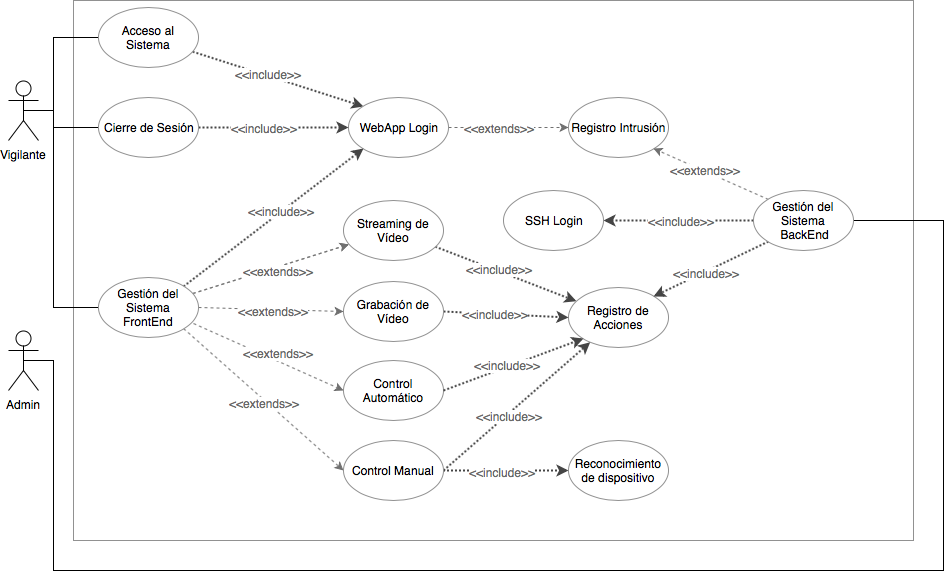
\includegraphics[width=1.35\textwidth]{caseUseDiag}
	\caption[Diagrama de Casos de Uso]{Diagrama de Casos de Uso.}\label{fig:caseUseDiag}
\end{figure}

\end{landscape}
\clearpage
}


\subsection{Actores}

\begin{itemize}
\item \textbf{Vigilante:} Actor a cargo de la gestión del sistema en producción. Interactúa con el FrontEnd.
\item \textbf{Admin:} Actor a cargo de la gestión del sistema en desarrollo o en caso de resolución de problemas en producción. Interactúa con el BackEnd.
\end{itemize}

\subsection{Casos de Uso}

\begin{table}
	\begin{center}
	\rowcolors {2}{gray!15}{}
		\begin{tabular}{m{3cm}  m{10cm}}\hline
			\toprule
			\textbf{CU-01} & \textbf{Acceso al sistema}\\
			\otoprule
			\textbf{Actor} & Vigilante\\
			\textbf{Requisitos asociados} & RF-1, RF-5\\
			\textbf{Descripción} & Permite al usuario iniciar sesión en el sistema vía web.\\
			\textbf{Precondiciones} & La base de datos está activa. El usuario dispone de cuenta activa.\\
			\textbf{Acciones} & \begin{enumerate}
											\item El usuario accede a la página web.
											\item El usuario introduce sus credenciales.
											\item Se muestra la página principal con el logo y los botones asociados al streaming de vídeo.
											\end{enumerate}\\
			
			\textbf{Postcondición} & El sistema habrá asignado al usuario el \emph{drone} correspondiente. \\
			\textbf{Excepciones} & \begin{itemize}
												\item Contraseña/Usuario incorrectos (mensaje).
												\item No existen \emph{drones} asociados (mensaje).
												\end{itemize}\\
			\textbf{Importancia} & Alta.\\
			\hline
			\bottomrule
		\end{tabular}
		\caption{CU-01. Acceso al sistema}
		\label{tb:CU01}
	\end{center}
\end{table}



\begin{table}
	\begin{center}
	\rowcolors {2}{gray!15}{}
		\begin{tabular}{m{3cm}  m{10cm}}\hline
			\toprule
			\textbf{CU-02} & \textbf{Cierre de sesión}\\
			\otoprule
			\textbf{Actor} & Vigilante\\
			\textbf{Requisitos asociados} & RF-2, RF-5\\
			\textbf{Descripción} & Permite al usuario cerrar sesión en el sistema vía web.\\
			\textbf{Precondiciones} & La base de datos está activa. El usuario dispone de cuenta activa. El usuario tiene iniciada una sesión.\\
			\textbf{Acciones} & \begin{enumerate}
											\item El usuario accede a la aplicación web.
											\item El usuario pulsa sobre el enlace `Logout' situado en la parte superior izquierda.
											\item Se muestra la página de inicio de sesión con un mensaje de despedida.
											\end{enumerate}\\
			
			\textbf{Postcondición} & El sistema habrá dado por cerrada la sesión de usuario. Se redirige al usuario a la página de inicio de sesión.\\
			\textbf{Excepciones} & El usuario no tenía sesión activa. (redirección a login).\\
			\textbf{Importancia} & Alta.\\
			\hline
			\bottomrule
		\end{tabular}
		\caption{CU-02. Cierre de sesión}
		\label{tb:CU02}
	\end{center}
\end{table}

\begin{table}
	\begin{center}
	\rowcolors {2}{gray!15}{}
		\begin{tabular}{m{3cm}  m{10cm}}\hline
			\toprule
			\textbf{CU-03} & \textbf{Gestión del sistema}\\
			\otoprule
			\textbf{Actor} & Vigilante\\
			\textbf{Requisitos asociados} & RF-1, RF-3\\
			\textbf{Descripción} & Permite al usuario gestionar las acciones del \emph{drone} vía web.\\
			\textbf{Precondiciones} & La base de datos está activa. El usuario dispone de cuenta activa. El usuario tiene iniciada una sesión. El usuario tiene asignado un \emph{drone}.\\
			\textbf{Acciones} & \begin{enumerate}
											\item El usuario conecta un dispositivo con el número de canales necesarios. 
											\item Se informa sobre el reconocimiento de dicho dispositivo y se muestran los valores de los canales activos.
											\item Se muestra el botón de activación del control manual.
											\end{enumerate}\\
			
			\textbf{Postcondición} & El sistema habrá asignado al usuario el \emph{drone} correspondiente. La aplicación web habrá reconocido el dispositivo conectado. Se dará la posibilidad de activar el control manual.\\
			\textbf{Excepciones} & Dispositivo no reconocido.\\
			\textbf{Importancia} & Alta.\\
			\hline
			\bottomrule
		\end{tabular}
		\caption{CU-03. Gestión del sistema}
		\label{tb:CU03}
	\end{center}
\end{table}


\begin{table}
	\begin{center}
	\rowcolors {2}{gray!15}{}
		\begin{tabular}{m{3cm}  m{10cm}}\hline
			\toprule
			\textbf{CU-04} & \textbf{Gestión del streaming de vídeo}\\
			\otoprule
			\textbf{Actor} & Vigilante\\
			\textbf{Requisitos asociados} & RF-3, RF-3.1 RF-3.5\\
			\textbf{Descripción} & Permite al usuario activar/desactivar el feed de vídeo proveniente del \emph{drone}.\\
			\textbf{Precondiciones} & La base de datos está activa. El usuario dispone de cuenta activa. El usuario tiene iniciada una sesión. El usuario tiene asignado un \emph{drone}.\\
			\textbf{Acciones} & \item El usuario pulsa sobre el botón `Start/Stop Streaming'\\
			
			\textbf{Postcondición} & La aplicación web inicia/detiene el vídeo.\\
			\textbf{Excepciones} &  \emph{Drone} no disponible (mensaje).\\
			\textbf{Importancia} & Alta.\\
			\hline
			\bottomrule
		\end{tabular}
		\caption{CU-04. Gestión del streaming de vídeo}
		\label{tb:CU04}
	\end{center}
\end{table}


\begin{table}
	\begin{center}
	\rowcolors {2}{gray!15}{}
		\begin{tabular}{m{3cm}  m{10cm}}\hline
			\toprule
			\textbf{CU-05} & \textbf{Grabación de vídeo}\\
			\otoprule
			\textbf{Actor} & Vigilante\\
			\textbf{Requisitos asociados} & RF-3, RF-3.2 RF-3.5\\
			\textbf{Descripción} & Permite al usuario grabar el feed de vídeo proveniente del \emph{drone}.\\
			\textbf{Precondiciones} & La base de datos está activa. El usuario dispone de cuenta activa. El usuario tiene iniciada una sesión. El usuario tiene asignado un \emph{drone}.\\
			\textbf{Acciones} & \item El usuario pulsa sobre el botón `Record Video'\\
			
			\textbf{Postcondición} & La aplicación web comienza con la grabación del feed de vídeo.\\
			\textbf{Excepciones} &\item Feed de vídeo no disponible (mensaje).\\
			\textbf{Importancia} & Baja.\\
			\hline
			\bottomrule
		\end{tabular}
		\caption{CU-05. Grabación de vídeo}
		\label{tb:CU05}
	\end{center}
\end{table}

\begin{table}
	\begin{center}
	\rowcolors {2}{gray!15}{}
		\begin{tabular}{m{3cm}  m{10cm}}\hline
			\toprule
			\textbf{CU-06} & \textbf{Control manual del \emph{drone}}\\
			\otoprule
			\textbf{Actor} & Vigilante\\
			\textbf{Requisitos asociados} & RF-3, RF-3.3 RF-3.5, RF-3.3.1, RF-6\\
			\textbf{Descripción} & Permite al usuario controlar el \emph{drone} de forma manual.\\
			\textbf{Precondiciones} & La base de datos está activa. El usuario dispone de cuenta activa. El usuario tiene iniciada una sesión. El usuario tiene asignado un \emph{drone}. El usuario ha conectado un dispositivo adecuado.\\
			\textbf{Acciones} & El usuario pulsa sobre el botón `Enable/Disable Manual'\\
											
			\textbf{Postcondición} & La aplicación web solicita la activación del control manual al sistema. El sistema se conecta al \emph{drone} y transmite la información proveniente de la aplicación web.\\
			\textbf{Excepciones} & \emph{Drone} no disponible (mensaje).\\
			\textbf{Importancia} & Alta.\\
			\hline
			\bottomrule
		\end{tabular}
		\caption{CU-06. Control manual}
		\label{tb:CU06}
	\end{center}
\end{table}

\begin{table}
	\begin{center}
	\rowcolors {2}{gray!15}{}
		\begin{tabular}{m{3cm}  m{10cm}}\hline
			\toprule
			\textbf{CU-07} & \textbf{Gestión de controles automáticos}\\
			\otoprule
			\textbf{Actor} & Vigilante\\
			\textbf{Requisitos asociados} & RF-3, RF-3.4 RF-3.5\\
			\textbf{Descripción} & Permite al usuario activar/desactivar los mecanismos de control automatizado del \emph{drone}.\\
			\textbf{Precondiciones} & La base de datos está activa. El usuario dispone de cuenta activa. El usuario tiene iniciada una sesión. El usuario tiene asignado un \emph{drone}.\\
			\textbf{Acciones} & \begin{enumerate}
											\item El usuario selecciona los mecanismos de control automatizado que desea emplear.
											\item El usuario pulsa sobre el botón `Enable auto'
											\end{enumerate}\\
											
			\textbf{Postcondición} & La aplicación web solicita la activación de los controles automatizados al sistema. El sistema se conecta al \emph{drone} y transmite la información proveniente de la aplicación web.\\
			\textbf{Excepciones} & \begin{itemize}
												\item \emph{Drone} no disponible (mensaje).
												\item Mecanismo automatizado no reconocido (mensaje).
												\end{itemize}\\
			\textbf{Importancia} & Media.\\
			\hline
			\bottomrule
		\end{tabular}
		\caption{CU-07. Gestión de controles automáticos}
		\label{tb:CU07}
	\end{center}
\end{table}


\begin{table}
	\begin{center}
	\rowcolors {2}{gray!15}{}
		\begin{tabular}{m{3cm}  m{10cm}}\hline
			\toprule
			\textbf{CU-08} & \textbf{Gestión del \emph{backend}}\\
			\otoprule
			\textbf{Actor} & Admin\\
			\textbf{Requisitos asociados} & RF-4, RF-5\\
			\textbf{Descripción} & Permite al usuario gestionar el equipo que controla el \emph{drone}.\\
			\textbf{Precondiciones} & El usuario dispone de credenciales de acceso al sistema.\\
			\textbf{Acciones} & \begin{enumerate}
											\item El usuario inicia sesión en el sistema.
											\item Se informa sobre el registro de intentos de acceso no autorizado.
											\item Se muestra el \emph{prompt} del sistema a la espera de órdenes.
											\end{enumerate}\\
			
			\textbf{Postcondición} & El sistema operativo habrá registrado el inicio de sesión del usuario. El sistema operativo habrá iniciado sesión con el usuario solicitado.\\
			\textbf{Excepciones} & Acceso denegado, pubkey. (mensaje)\\
			\textbf{Importancia} & Alta.\\
			\hline
			\bottomrule
		\end{tabular}
		\caption{CU-08. Gestión del \emph{backend}.}
		\label{tb:CU08}
	\end{center}
\end{table}


